\section{Lean Theorem Prover}

A medida que las matemáticas se vuelven más técnicas y especializadas, verificar con rigor las demostraciones formales es una tarea cada vez más costosa. Con la motivación de facilitarla, en las últimas décadas ha surgido un interés por la verificación computacional de teoremas, dando lugar al desarrollo de sistemas como Lean, Coq o Isabelle.

Dentro de este campo, distinguimos dos tipos de sistemas de verificación formal: interactivos (ITP), que proporcionan un entorno en el que usuario guía el proceso de la demostración paso a paso, centrándose en el aspecto de \quotes{verificación}, y automáticos (ATP), que buscan completar demostraciones de manera completamente autónoma \cite[Sección~1]{avigad2024theorem}.

En este trabajo nos centraremos en el uso de \textbf{Lean Theorem Prover}, introducido en 2013 por Leonardo de Moura desde Microsoft Research. Se trata de un verificador cuyo objetivo es reducir la distancia entre demostraciones asistidas y automatizadas, combinando un lenguaje basado en la teoría de tipos dependientes con herramientas que permiten delegar sub-problemas sencillos al sistema

Aunque aquí nos limitaremos a su uso como asistente de demostración, Lean es también un lenguaje de programación funcional completo, lo que ofrece amplias posibilidades de personalización y automatización al usuario \cite[Sección~1]{avigad2024theorem}.

En este sistema, es posible definir objetos matemáticos, especificar propiedades sobre ellos y demostrar que dichas propiedades se cumplen. Esta tarea se ve facilitada por \textit{Mathlib}, una extensa biblioteca de matemáticas formalizadas en Lean desarrollada de manera colaborativa por una comunidad activa y en constante crecimiento \cite{mathlib}.

Las demostraciones son verificadas automáticamente por el núcleo lógico de Lean, que garantiza su corrección mediante un sistema de tipos expresivo y riguroso. La fiabilidad de Lean como asistente de demostración reside precisamente en la simplicidad y robustez de este núcleo \cite{bailey2024type}.

En esta sección seguiremos principalmente el manual en línea \textit{Theorem Proving in Lean 4}~\cite{avigad2024theorem} que es una versión actualizada del libro \textit{Theorem Proving in Lean}~\cite{avigad2021theorem} publicado en 2021 para adaptarse a la nueva versión de Lean. A nivel teórico, no existe una gran diferencia entre los dos, por lo que ambas referencias son válidas para comprender los fundamentos que exponemos aquí.


\subsection{La teoría de tipos de Lean}

La teoría de conjuntos de Zermelo-Fraenkel con el axioma de elección (ZFC) es la base fundacional elegida para formalizar la mayoría de las matemáticas que conocemos. En este marco, todos los objetos matemáticos (números, funciones, estructuras algebraicas, etc.) pueden representarse como conjuntos, construidos a partir de unos pocos axiomas básicos.

Sin embargo, este sistema carece de una estructura interna diferenciada: todo objeto matemático, como un número, una función o incluso una colección de funciones son, en última instancia, conjuntos. Para lograr una representación más clara y diferenciada de los objetos matemáticos, Lean utiliza, en su lugar, un sistema basado en tipos. Además, este enfoque nos ofrece la posibilidad de establecer una correspondencia entre programas y demostraciones matemáticas, conocida como la correspondencia de Curry-Howard\footnote{La correspondencia de Curry-Howard establece una relación entre lógica y programación; permite entender como pueden ser equivalentes \quotes{demostrar una proposición} y \quotes{construir un término de cierto tipo}. Veremos qué quiere decir esto en la práctica más adelante, pero las ideas más profundas, que quedan fuera del alcance de este trabajo, se exponen detalladamente en \cite{sorensen2006lectures}.}.

En particular, Lean se fundamenta en el \textit{Cálculo de Construcciones Inductivas}, una extensión del cálculo de tipos dependientes que incorpora tipos inductivos y una jerarquía numerable no acumulativa de universos \cite{coquand1986calculus}. Aunque no es necesario entender este sistema para utilizar Lean como asistente de demostración, a continuación daremos una breve explicación de los conceptos fundamentales.

En esta sección, veremos varios fragmentos de código en Lean. Lean cuenta con un compilador interactivo que procesa cada línea cuando el cursor se encuentra sobre ella, mostrando el resultado por pantalla. A partir de ahora, los comentarios que acompañan al código reflejan la salida que Lean devuelve en cada línea. Los comentarios en Lean se escriben empezando con doble guión ($--$) y están en color gris.

\subsubsection{Teoría de tipos}

Empecemos por lo más básico: la teoría de tipos. Cambiamos el foco de \quotes{cada objeto es un conjunto }, propio de ZFC, a \quotes{cada objeto es un término con un tipo asociado}. Esto nos permite estructurar con mayor claridad los objetos matemáticos y sus relaciones.

Por ejemplo, $3$ es un término de tipo \quotes{natural} ($\mathbb{N}$), mientras que \quotes{true} es un término de tipo \quotes{booleano}. En Lean podemos comprobar el tipo de estas expresiones utilizando el comando \bluecode{\#check}\footnote{En Lean, podemos escribir $\mathbb{N}$ escribiendo \code{$\backslash$nat} en el editor y luego pulsando espacio. En general, escribiremos los símbolos matemáticos de esta forma. Una lista comprensiva con los símbolos utilizados en el proyecto y sus respectivos comandos se puede encontrar en (un anexo)}:


\begin{lstlisting}
  #check 3    -- 3 : ℕ 
  #check true   -- Bool.true : Bool
\end{lstlisting}

Como en este ejemplo, en Lean utilizamos el símbolo $:$ para describir la información sobre el tipado. Es decir, si $x$ es un término de tipo $X$, escribimos $x : X$.

Por otro lado, un tipo, como es $\mathbb{N}$, también es un término. Podemos comprobar su tipo:

\begin{lstlisting}
  #check ℕ    -- ℕ : Type
\end{lstlisting}

En Lean, los tipos tienen su propio tipo, que recibe el nombre de \code{Type}. Esto nos permite definir nuevos tipos. Podemos utilizar el comando \bluecode{variable} para definir objetos en nuestro código\footnote{Veremos este comando en detalle más adelante}.

\begin{lstlisting}
  variable (X : Type)
  #check X    -- X : Type
  variable (x : X)
  #check x    -- x : X
\end{lstlisting}

Ahora, podemos combinar distintos tipos para obtener tipos más complejos. Sean $X$ e $Y$ dos tipos. Podemos considerar el tipo $X \times Y$, que denota los pares formados por un elemento de $X$ y otro de $Y$. El tipo que más utilizaremos es $X \to Y$, que denota las funciones de $X$ en $Y$. Escribimos esto en Lean.

\begin{lstlisting}
  variable (X Y : Type)
  #check X × Y    -- X × Y : Type
  variable (x : X) (y : Y)
  #check (x, y)    -- (x, y) : X × Y
  
  #check X → Y    -- X → Y : Type
  variable (f : X → Y)
  #check f    -- f : X → Y
\end{lstlisting}

Por otro lado, a partir de la yuxtaposición de términos simples, podemos formar términos más complejos. En Lean, las reglas de tipado dictan el tipo de estos nuevos términos obtenidos. Por ejemplo, si $x$ es de tipo $X$ y $f$ es de tipo $A \to B$, como en el ejemplo anterior, entonces $f x$ tiene tipo $B$. En efecto:

\begin{lstlisting}
  #check f x    -- f x : Y
\end{lstlisting}

La capacidad de Lean para identificar el tipo de un término sin necesidad de que el usuario lo especifique se conoce como \textbf{inferencia de tipos}. Como veremos más adelante, este proceso ocurre de manera automática en su núcleo y es el aspecto crucial de la verificación de demostraciones.

\subsubsection{Teoría de tipos dependientes}

Para poder expresar los distintos objetos matemáticos en esta teoría, es importante que un tipo no sea necesariamente estático, sino que pueda depender de otros términos.

Por ejemplo, \code{Fin} es un tipo en Lean que describe los números naturales menores que otro número natural dado. Precisamente, no tiene sentido afirmar que un término tiene tipo \code{Fin}, porque \code{Fin} depende de este número dado: un término de tipo \code{$\mathbb{N}$}. En efecto,

\begin{lstlisting}
  #check Fin    -- Fin (n : ℕ) : Type
  #check Fin 5    -- Fin 5 : Type
\end{lstlisting}

Decimos que \code{Fin} es un tipo dependiente, porque depende del valor de n. Lean admite, por tanto, tipos dependientes en su teoría.

\subsubsection{Cálculo de Construcciones}

El Cálculo de Construcciones es una extensión del Cálculo Lambda con tipos \cite{coquand1986calculus}. El Cálculo Lambda, introducido por Alonzo Church en los años 1930, es un sistema formal en el que todos los términos se ven como funciones (o abstracciones) y se operan entre sí mediante aplicación de funciones (el uso de una función sobre un argumento) \cite{pierce2002types}. A pesar de su simplicidad, este sistema se ha convertido en la base formal de muchos lenguajes de programación modernos.

Por ejemplo, una función válida podría ser $n \mapsto 2n : \mathbb{N} \rightarrow \mathbb{N}$, que representa una función que, al ser aplicada a un número natural, devuelve el número multiplicado por dos.

En Lean, definimos funciones utilizando el comando \code{fun}\footnote{En la versión anterior de Lean, se utilizaba la notación \code{$\lambda$ n, 2 * n}, más similar a la del Cálculo Lambda, sin embargo en esta última versión se ha cambiado a \code{fun n $\mapsto$ 2 * n} para mejorar la legibilidad del código.}, por ejemplo\footnote{Estudiaremos el comando \bluecode{def} en detalle más adelante.}:

\begin{lstlisting}
  def f : ℕ → ℕ := fun n ↦ 2 * n
\end{lstlisting}

Además, se puede definir una reducción sobre este tipo de términos: el término formado por la anterior función aplicada a $3$, $(n \mapsto 2n)3$, se puede reducir a $2 \cdot 3$ por aplicación funcional, y luego a $6$ por definición de la multiplicación.

Podemos comprobar el resultado de esta reducción utilizando el comando \bluecode{\#eval}.

\begin{lstlisting}
  #eval f 3    -- 6
\end{lstlisting}

Diremos que dos términos que pueden reducirse de esta manera al mismo valor son \textbf{iguales por definición}. Lean trata términos que sean iguales por definición como literalmente iguales, como veremos más adelante. En la siguiente sección, utilizaremos la noción de equivalencia por definición con frecuencia.

\subsubsection{Jerarquía de universos}

Puesto que en la teoría de tipos cada elemento tiene un tipo, también el tipo \code{Type} tiene un tipo asociado: el tipo \code{Type 1}. A su vez, \code{Type 1} tiene tipo \code{Type 2} y, en general, \code{Type n} tiene tipo \code{Type n+1} para cada $n$, formando una jerarquía numerable de tipos que llamaremos \textbf{universos}.

Esta jerarquía es no acumulativa, lo que significa que si \code{A : Type n}, no se asume en general que \code{A : Type (n+1)}. Esta propiedad evita que ocurran conversiones implícitas y facilita la inferencia de tipos de Lean. Sin embargo, en la práctica Lean se encarga de realizar ciertas conversiones de manera automática, por lo que rara vez es necesario trabajar explícitamente con los universos.

\subsubsection{Tipos inductivos}

En Lean, la gran mayoría de tipos son instancias de una familia de tipos conocidos como \textbf{tipos inductivos}. Un tipo inductivo es una estructura formada por una lista finita de constructores, cada uno con su tipo correspondiente. Cada constructor describe una forma válida de construir un término de este nuevo tipo.

En Lean, definimos un tipo inductivo utilizando la palabra clave \bluecode{inductive}\footnote{Aunque en Lean los tipos inductivos se introducen como una construcción primitiva del lenguaje, pueden definirse de manera equivalente sólo en términos de tipos dependientes. Esta reducción se explora formalmente en \cite{carneiro2019type}.}.

\begin{lstlisting}
  inductive Foo where
    | constructor₁ : ... → Foo
    | constructor₂ : ... → Foo
    ...
    | constructorₙ : ... → Foo
\end{lstlisting}

Un ejemplo clásico de definición inductiva es el conjunto de los números naturales, $\mathbb{N}$. En Lean, podríamos describir el tipo \code{Nat} de los números naturales como

\begin{lstlisting}
  inductive Nat where
    | zero : Nat
    | succ : Nat → Nat
\end{lstlisting}

Internamente, la declaración \bluecode{inductive} genera automáticamente una colección de axiomas que definen el tipo:

\begin{itemize}
  \item Una constante, \code{Nat}, que representa el nuevo tipo.
  \item Una serie de reglas de introducción o constructores, que indican las posibles formas de construir términos del nuevo tipo. 
  \item Una regla de eliminación, \code{Nat.rec}, que indica la forma de \quotes{usar} un término de este tipo\footnote{El comando \bluecode{\#print} muestra la definición completa del objeto, a diferencia de \bluecode{\#check}, que solo muestra su tipo.}.
  \begin{lstlisting}
  #print Nat.rec
      -- recursor Nat.rec.{u}  :  {motive : ℕ → Sort u} → motive Nat.zero → ((n : ℕ) → motive n → motive n.succ) → (t : ℕ) → motive t\end{lstlisting}\end{itemize}

Es decir, \bluecode{inductive} puede verse como \textit{azúcar sintáctico} que genera automáticamente el siguiente código en Lean\footnote{Estudiaremos el comando \bluecode{axiom} en detalle más adelante.}:

\begin{lstlisting}
  axiom (Nat : Type)
  axiom (zero : Nat)
  axiom (succ : Nat → Nat)
  axiom (Nat.rec : {motive : Nat → Sort u} → motive Nat.zero →
    ((n : Nat) → motive n → motive Nat.succ n) → (t : Nat) → motive t)
\end{lstlisting}

Este último objeto, \code{Nat.rec}, codifica el principio de inducción sobre los naturales\footnote{\code{Nat.rec} es un tipo que depende de \code{motive}, que es una propiedad cualquiera sobre los naturales. \code{Nat.rec} nos dice que si se cumple \code{motive} para \code{Nat.zero} (\code{motive Nat.zero}), entonces si para cada \code{n} (\code{n : Nat}) que cumpla \code{motive} (\code{motive n}) se tiene que \code{n+1} cumple \code{motive} (\code{motive Nat.succ n}), entonces se cumple \code{motive} para cualquier \code{n} (\code{(t : Nat) → motive t}).}. Este principio se utiliza implícitamente en muchas definiciones por casos, como por ejemplo:

\begin{lstlisting}
  def add (m n : Nat) : Nat :=
    match n with
    | Nat.zero   => m
    | Nat.succ n => Nat.succ (add m n)
\end{lstlisting}

En esta definición, utilizamos la expresión \code{match n with} para distinguir los dos posibles casos de un número natural: \code{zero} y \code{succ n}. Internamente, Lean compila esta expresión como una aplicación de \code{Nat.rec}. Veremos más adelante cómo este principio de inducción puede utilizarse no solo para definir funciones, sino también para probar propiedades sobre todos los términos de un tipo inductivo.

Finalmente, mediante los tipos inductivos es posible definir los conectores lógicos (negación, conjunción, disyunción e implicación). Esto constituye otra gran diferencia entre la teoría de conjuntos y el cálculo de construcciones inductivas. Para utilizar la teoría de conjuntos, es necesario haber desarrollado previamente la lógica (de primer orden). De esta manera, las demostraciones formales no constituyen objetos matemáticos, sino que viven exclusivamente en el plano meta-teórico.

En el cálculo de construcciones inductivas, en cambio, la lógica se expresa dentro de la misma teoría, y las demostraciones son objetos matemáticos que viven dentro de ella.

\subsubsection{Las demostraciones como objeto matemático}

Las proposiciones, como cualquier otro objeto en esta teoría, son términos con un tipo asociado. En Lean, este tipo recibe el nombre de \code{Prop}.

\begin{lstlisting}
  #check Prop    -- Prop : Type
  variable (P : Prop)
  #check P    -- P : Prop
  #print True    -- inductive True : Prop
  #check ¬ P    -- ¬ P : Prop
\end{lstlisting}

En Lean, interpretamos los objetos de tipo \code{Prop} como tipos en sí mismos. En particular, una proposición \code{p : Prop} es el tipo de las demostraciones de \code{p}. Por tanto, una expresión de la forma \code{h : p} quiere decir que \code{h} es una demostración de \code{p}. Tiene entonces sentido decir que una proposición \code{p} es verdadera si podemos construir término de tipo \code{p}.

\begin{lstlisting}
  variable (p : Prop)
  variable (h : p)
  #check h    -- h : p
\end{lstlisting}

Esto, junto con la teoría de tipos dependientes, nos proporciona una forma de definir cualquier resultado matemático: por ejemplo, \quotes{ser par} es una propiedad que depende de un número natural $n$, por lo que podríamos describirlo mediante \code{es\_par : $\mathbb{N} \to$ Prop}. Para cada \code{n} natural, obtenemos un término de tipo \code{Prop}.

\begin{lstlisting}
  def es_par : ℕ → Prop := ...
  #check es_par    -- es_par : ℕ → Prop
  #check es_par 3    -- es_par 3 : Prop
\end{lstlisting}

En este caso, un término de tipo \code{es\_par n} será una prueba de que \code{n} es par.

Además, si \code{p : Prop} es una proposición, Lean reconoce cualesquiera dos elementos de tipo \code{p} (\code{h1 h2 : p}) como iguales por definición: no importa qué prueba concreta tengamos, sólo importa su existencia. Esto se conoce como \quotes{irrelevacia de las demostraciones} (\textit{proof irrelevance}).

Esta propiedad tiene ventajas prácticas. Por ejemplo, si demostramos una existencia (una proposición del estilo $\exists x, P(x)$) de dos maneras distintas utilizando dos valores diferentes, Lean identificará ambas pruebas, por lo que al extraer de $\exists x, P(x)$ un valor $x$ con $P(x)$, este valor será independiente de la demostración utilizada. Sin embargo, esto también tiene la desventaja de que este tipo de pruebas no son constructivas: no es posible recuperar exactamente el valor que utilizamos para completar la demostración.

También por esta propiedad, dadas dos proposiciones \code{p q : Prop}, podemos identificar los términos de tipo \code{Implies p q} con los términos de tipo \code{p $\to$ q}; si \code{h : Implies p q}, entonces \code{h} es una prueba de que \code{p} implica \code{q}, y por tanto podemos verlo como una función que, dada una prueba de \code{p}, devuelve una prueba de \code{q}. El conector \code{Implies} es por tanto redundante, y en lo que sigue utilizaremos sólo la expresión \code{$\to$}.

En resumen, para poder expresar un resultado matemático en este lenguaje, tenemos que escribir un término de la forma \code{p : Prop}. Para probar que el resultado es cierto, debemos construir un término \code{h : p}. El trabajo de Lean como asistente de demostración es verificar que el término \code{h} está bien construido y tiene el tipo correcto.


\subsection{¿Por qué fiarnos de Lean?}

Ahora que hemos descrito la manera en la que un resultado se considera demostrado en Lean, tiene sentido hacerse la pregunta: ¿por qué deberíamos fiarnos de la inferencia de tipos de Lean? ¿Qué garantías tenemos de que las demostraciones que Lean acepta, son realmente correctas? 

Como hemos señalado, demostrar un resultado en Lean consiste en construir correctamente un término que tiene un determinado tipo. Este proceso es análogo al de verificar programas: se trata de comprobar que un término está bien formado (siguiendo unas reglas concretas) y satisface una especificación dada, expresada como un tipo. Esta tarea recae sobre el núcleo (o \textit{kernel}) de Lean, un pequeño programa que contiene la implementación mínima de la lógica interna de Lean.

El resto de componentes de Lean con el que interactuamos para construir demostraciones (como por ejemplo las tácticas que veremos después) devuelven construcciones expresadas en el lenguaje del kernel de Lean \cite{bailey2024type}. Esto quiere decir que confiar en Lean realmente se reduce a confiar en su kernel\footnote{Esta idea se conoce como \textit{criterio de de Bruijn}, que propone que un verificador formal debe producir sus pruebas en el lenguaje de un núcleo pequeño, incluso aunque utilicen otros métodos más complicados para construir dichas pruebas a priori \cite{bailey2024type}.}.

Ahora, ¿por qué nos fiamos del kernel de Lean? Gracias a que el kernel es pequeño y está aislado del resto del sistema, es posible escribir implementaciones independientes del mismo que verifiquen de manera autónoma las demostraciones aceptadas por Lean. Lean permite exportar estas demostraciones en un formato intermedio que contiene toda la información necesaria para reconstruirlas y validarlas externamente. Además, puesto que este formato modular, es posible validar solo ciertos aspectos concretos del kernel \cite{bailey2024type}. Por ejemplo, en \cite{carneiro2024lean4lean}, Carneiro describe una nueva implementación externa del verificador de tipos de Lean 4, escrita en el propio lenguaje Lean y capaz de verificar toda la biblioteca de \textit{Mathlib}.



\subsection{Demostraciones en Lean}

Hasta ahora, hemos explorado la teoría de tipos dependientes sobre la que se construye Lean, así como los fundamentos que garantizan la corrección de sus demostraciones. Pasamos por tanto a un enfoque más práctico: ¿cómo escribimos matemáticas en Lean?

Recordemos que formalizar un resultado en Lean no consiste solo en escribir su enunciado, sino también en construir una demostración paso a paso, sin omisiones y con total precisión. Aquí, nunca nos basta con escribir \quotes{trivial} cuando creamos que algo ya deberíamos poder saberlo: necesitamos convencer al sistema de que cada paso es válido.

Esta sección está dedicada a aprender a escribir demostraciones en Lean. Veremos cómo introducir nuevos objetos en nuestros contexto, como enunciar proposiciones y cómo construir demostraciones interactuando con Lean. También presentaremos algunas herramientas de automatización y métodos para poder apoyarnos en la librería de Mathlib.

\subsubsection{Axiomas, definiciones y variables}

Antes de escribir demostraciones en cualquier sistema formal, necesitamos describir el \textbf{contexto} en el que trabajamos: el conjunto de objetos e hipótesis disponibles en un momento dado. Este contexto es dinámico y se va ampliando a medida que introducimos nuevos elementos.

En Lean ocurre exactamente lo mismo. El sistema mantiene y actualiza este contexto constantemente para comprobar que cada expresión está bien formada y tiene el tipo esperado.

Podemos introducir nueva información en el contexto de distintas formas. Distinguimos entre axiomas, definiciones y variables, cada una con una función lógica distinta en el sistema.

\begin{itemize}
  \item \textbf{Axiomas}\footnote{En Lean 3, a este tipo de declaraciones se les llamaba \textit{constantes} y utilizaban el comando \bluecode{constant}.}
\end{itemize}

Permiten introducir hipótesis que se asumen sin demostración. En particular, escribir que x \quotes{es de tipo X} es también una hipótesis, por lo que los axiomas pueden utilizarse para introducir nuevos objetos\footnote{En este sentido decíamos que definir un tipo inductivo es análogo a escribir una colección de axiomas. \code{inductive Nat} se puede ver como una versión estructurada de \code{axiom Nat : Type}, \code{axiom zero : Nat}, \code{axiom succ : Nat to Nat}, etc.}. Por ejemplo:

\begin{lstlisting}
  axiom P : Prop
  axiom h : P → P
\end{lstlisting}

Estamos declarando una proposición $P$ y una prueba de que $P$ implica $P$.

\begin{lstlisting}
  axiom n : ℕ
  axiom hn : n > 2
\end{lstlisting}

Aquí estamos suponiendo que $n$ es un número natural mayor que $2$.

Así, los axiomas nos permiten fijar hechos en el contexto que queremos asumir como válidos a lo largo de nuestras demostraciones.


\begin{itemize}
  \item \textbf{Definiciones}
\end{itemize}

Introducen objetos nuevos a partir de otros ya conocidos. A diferencia de los axiomas, no  basta con indicar el tipo del nuevo objeto, sino que también hay que dar su construcción. Por ejemplo:

\begin{lstlisting}
  def f : ℕ → ℕ := fun n ↦ 2 * n
  def n : ℕ := 3
  def es_par : ℕ → Prop := fun n ↦ ∃ m, n = f m
\end{lstlisting}

Además, cuando el tipo puede inferirse a partir de la construcción, no es necesario indicarlo explícitamente:

\begin{lstlisting}
  def n := 3
  #check n    -- n : ℕ
\end{lstlisting}

\begin{itemize}
  \item \textbf{Variables}
\end{itemize}

En la mayoría de lenguajes de programación, estamos acostumbrados a que definir una variable implique asignarle un valor concreto. Sin embargo, en Lean las variables se comportan más bien como en lógica. Al introducir una variable $x$, lo que se introduce es un contexto universal: siempre que $x$ aparezca de forma libre, Lean interpretará que lo que sigue está cuantificado universalmente respecto a $x$. Por ejemplo\footnote{Las variables, a diferencia de los axiomas y las definiciones, se escriben entre paréntesis. Lo mismo ocurre con los argumentos que toman las proposiciones, como veremos más adelante. Esto está relacionado con la correspondencia de Curry–Howard: declarar una variable equivale a abstraer sobre ella, lo que corresponde a cuantificar universalmente.}:

\begin{lstlisting}
  variable (x : ℕ)
  axiom hx : x ≥ 0
  #print hx    -- axiom hx : ∀ (x : ℕ), x ≥ 0
\end{lstlisting}

\subsubsection{Proposiciones}

Además de introducir objetos, también queremos enunciar y demostrar proposiciones. En Lean, esto se hace del mismo modo que en otros sistemas formales: primero escribimos los resultados (como lemas o teoremas) formalmente, y después proporcionamos una demostración.

Como ya hemos visto, una proposición en Lean es un término de tipo \code{Prop}, y una demostración de \code{p : Prop} es simplemente un término de tipo \code{p}. Por tanto, demostrar una proposición no es diferente de definir un objeto; podemos utilizar \bluecode{def} para escribir resultados matemáticos. Por ejemplo:

\begin{lstlisting}
  def mi_prop : 1 > 0 := ...
\end{lstlisting}

Aquí estamos diciendo que \code{mi\_prop} es un objeto de tipo \code{1 > ~0}. Si en el lugar de \code{...} proporcionamos un término de tipo \code{1 > ~0}, habremos demostrado \code{mi\_prop}.

Sin embargo, para mayor claridad y estructura, Lean proporciona los comandos \bluecode{lemma} y \bluecode{theorem}. Ambos funcionan exactamente igual que \bluecode{def} y son intercambiables entre sí, pero facilitan la lectura del código indicando qué objetos son resultados matemáticos, y la jerarquía de importancia entre ellos. La sintaxis es la misma:

\begin{lstlisting}
  lemma my_lemma : 1 > 0 := ...
  theorem commutative_sum (a b : ℕ) : a + b = b + a := ...
\end{lstlisting}

Existe también el comando \bluecode{example}, que sirve para escribir demostraciones sin la necesidad de nombrar el resultado:

\begin{lstlisting}
  example (a b : ℕ) : a * b = b * a := ...
\end{lstlisting}

Este tipo de expresiones no amplían el contexto ni definen nuevos objetos; son simplemente comprobaciones locales. Pero veremos que nos pueden ser útiles en ciertas ocasiones.


\subsubsection{Demostraciones: el modo táctico}

Llegamos a la parte central de esta sección: \textbf{escribir demostraciones} en Lean. En general, hay dos formas de construir una demostración en Lean:

\begin{itemize}
  \item Mediante \textbf{términos}, es decir, escribiendo directamente una expresión del tipo deseado.
  \item Mediante el \textbf{modo táctico}, en el que una demostración se construye paso a paso usando instrucciones llamadas \textbf{tácticas}.
\end{itemize}

En este trabajo utilizaremos exclusivamente el modo táctico, ya que es el enfoque más práctico y más cercano a la forma en que razonamos al escribir demostraciones matemáticas en lenguaje natural. 

En una demostración informal, solemos avanzar mediante pasos lógicos encadenados: \quotes{supongamos que...}, \quotes{entonces...}, \quotes{por el lema..., se tiene...}. Cada uno de estos pasos se traduce en Lean mediante una táctica: una instrucción que modifica el estado de la demostración, ya sea introduciendo hipótesis, aplicando resultados conocidos, dividiendo el objetivo en partes más manejables, etc.

Además, el modo táctico nos permite trabajar de manera \textbf{interactiva} con Lean. Si escribimos un enunciado, e inmediatamente después de \code{:=} escribimos \bluecode{by}, estamos indicando a Lean que para la construcción de este término vamos a utilizar el modo táctico. Por ejemplo:

\begin{lstlisting}
  theorem and (p q : Prop) (hp : p) (hq : q) : p ∧ q := by
\end{lstlisting}

Estamos indicando que queremos construir un término de tipo \code{p $\land$ q} a partir de las hipótesis \code{hp : p} y \code{hq : q}, y que para esa construcción vamos a utilizar el modo táctico.

Internamente, Lean interpreta esto mediante la generación de un contexto local (nuestras hipótesis) y un \textbf{objetivo} (nuestra tesis), que consiste en construir el término del tipo esperado. Después de \bluecode{by}, podemos empezar a escribir tácticas, que Lean interpretará actualizando el contexto y el objetivo deseado.

Este objetivo aparece reflejado en el \textbf{InfoView}, una ventana que muestra el estado actual de nuestra demostración. Lean procesa línea a línea de forma automática, por lo que en cualquier momento podemos consultar el impacto de haber aplicado una táctica simplemente colocando el cursor sobre la línea de código correspondiente.

De hecho, en el InfoView también se muestran los resultados de las instrucciones que ya hemos visto como \bluecode{\#check}, \bluecode{\#print} o \bluecode{\#eval}.

\begin{figure}[h]
  \centering
  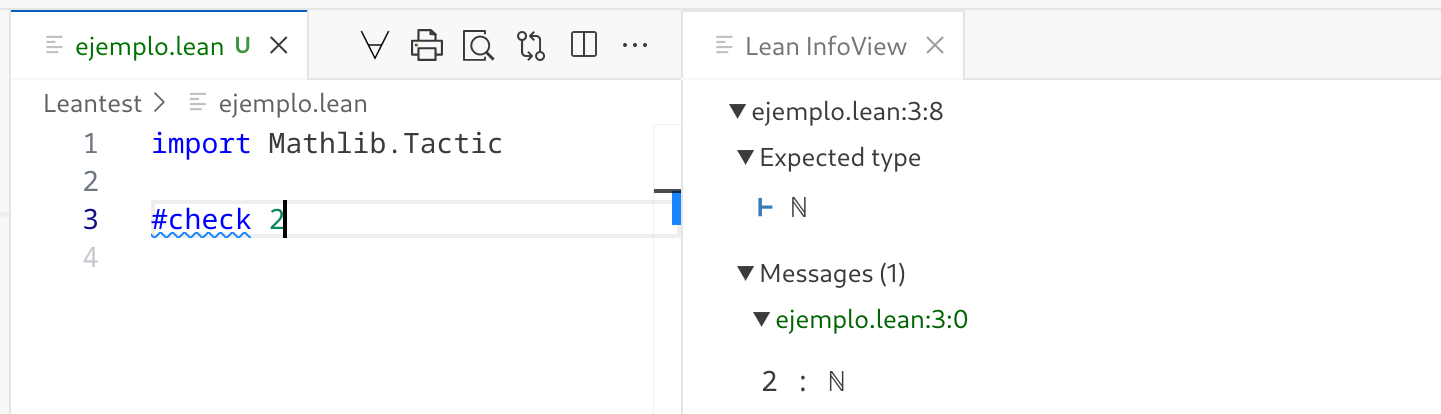
\includegraphics[width=1\textwidth]{figuras/check-example-light-version.png}
\end{figure}

En general, cuando escribamos en Lean, tendremos abierta esta ventana paralelamente a nuestro código, para poder ir viendo el progreso de nuestra demostración.

\begin{figure}[h]
  \centering
  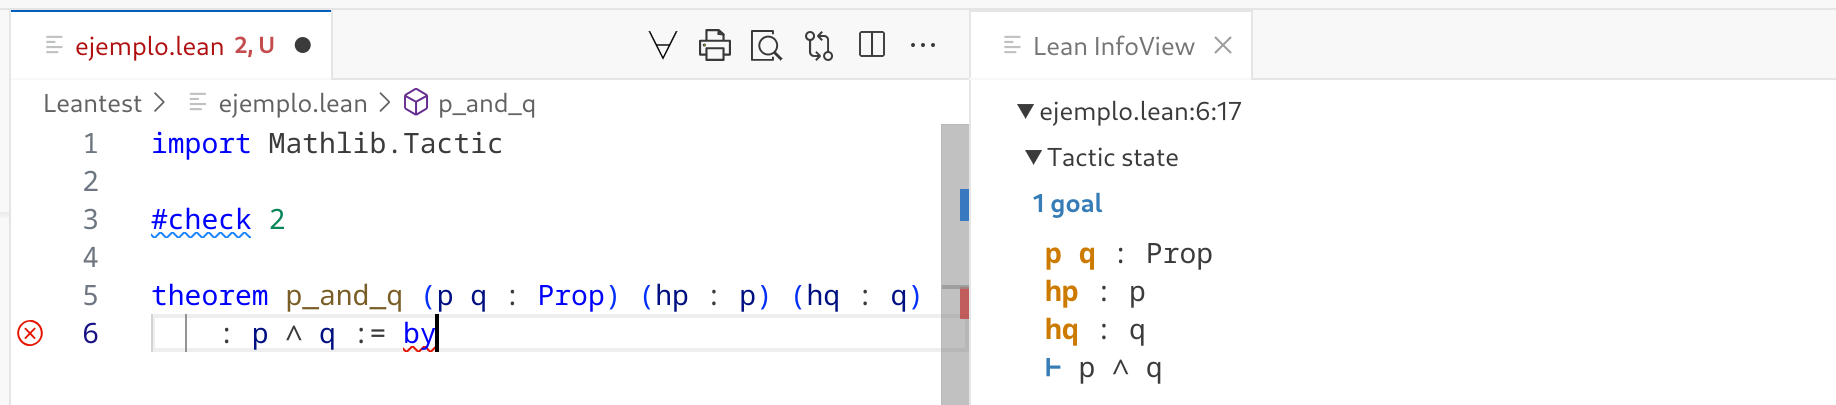
\includegraphics[width=1\textwidth]{figuras/theorem-example-light-version.png}
\end{figure}

Bajo el apartado \code{Tactic state}, podemos comprobar:

\begin{itemize}
  \item El número de tesis que nos quedan por demostrar (en este caso solo una: \bluecode{1 goal}).
  \item Nuestro contexto.
  \item La (o las) tesis, marcadas con el símbolo \bluecode{$\vdash$}.
\end{itemize}

A partir de este punto, podemos empezar a añadir las tácticas que van a construir nuestra demostración. Las tácticas se escriben una detrás de otra, separadas por punto y coma (\code{;}) o por saltos de línea.

Al escribir una táctica, el apartado \code{Tactic state} del InfoView se actualizará según corresponda. Cuando todas las tesis se hayan resueltos, el InfoView mostrará \bluecode{No goals}.

\begin{figure}[h]
  \centering
  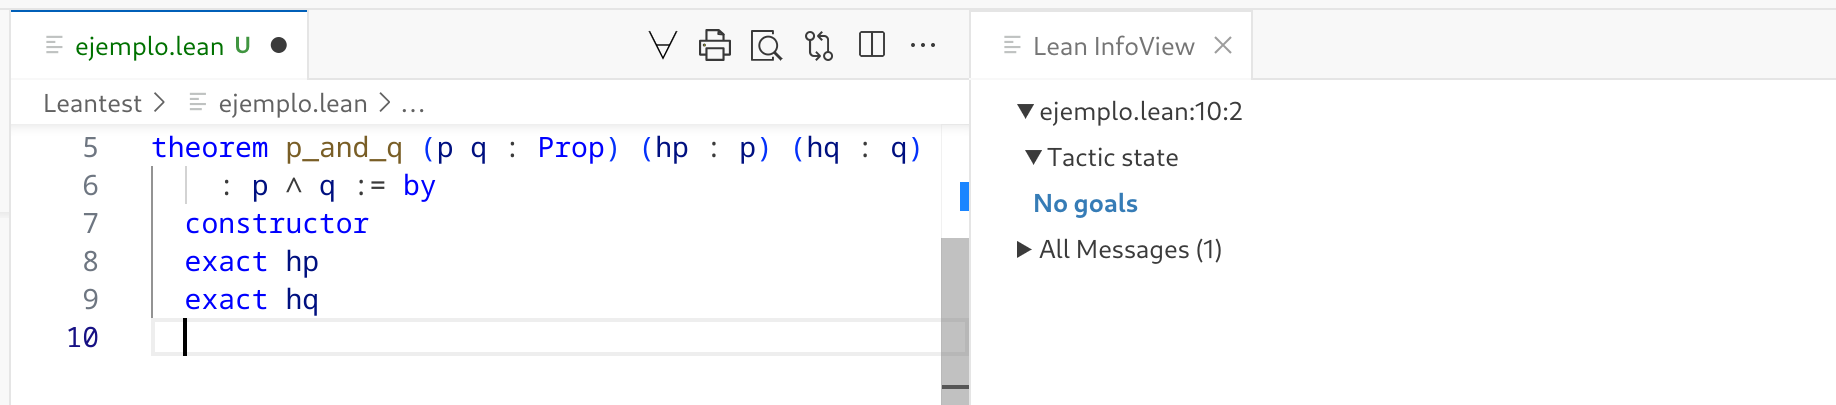
\includegraphics[width=1\textwidth]{figuras/no-goals-example-light-version.png}
\end{figure}

\subsubsection{Algunas tácticas básicas}

En esta sección veremos algunas de las tácticas más básicas y útiles para construir demostraciones en Lean. Veremos cómo se aplican y qué efecto tienen en el InfoView. El resto de tácticas que aparecen a lo largo del trabajo pueden consultarse en el Anexo (letra, probablemente la A).

Para poder utilizar las tácticas mencionadas a continuación, es necesario importar el módulo de Mathlib correspondiente al modo táctico con:

\begin{lstlisting}
  import Mathlib.Tactic
\end{lstlisting}

A partir de aquí, en lugar de mostrar capturas del InfoView, utilizaremos dos bloques de código en paralelo: el de la izquierda contiene el código de Lean, y el de la derecha representa el estado táctico que se vería en el InfoView si colocásemos el cursor en la última línea.

\vspace{1em}
\noindent\textbf{$~$ \largebluecode{intro}}

La táctica \bluecode{intro} introduce un nuevo objeto en el contexto, de manera similar a escribir \quotes{Supongamos que...} o \quotes{Sea...} en una demostración informal.

Es útil cuando el objetivo tiene la forma de una implicación o un cuantificador universal: transformamos la primera parte de la tesis en una nueva hipótesis y la segunda en la nueva tesis. Por ejemplo, para la implicación:


\begin{minipage}[t]{0.58\textwidth}
\begin{lstlisting}[language=lean]
  example (p : Prop) : p → p := by


~
\end{lstlisting}
\end{minipage}%
\hfill
\begin{minipage}[t]{0.40\textwidth}
\begin{lstlisting}[language=infoview]
  Tactic state
    ŋ1 goalŋ
    ħpħ : Prop
    ⊢ p → p
\end{lstlisting}
\end{minipage}
%
\noindent
\makebox[\textwidth]{$\downarrow$}
%
\begin{minipage}[t]{0.58\textwidth}
\begin{lstlisting}[language=lean]
  example (p : Prop) : p → p := by
    intro hp


~
\end{lstlisting}
\end{minipage}%
\hfill
\begin{minipage}[t]{0.40\textwidth}
\begin{lstlisting}[language=infoview]
  Tactic state
    ŋ1 goalŋ
    ħpħ : Prop
    ħhpħ : p
    ⊢ p
\end{lstlisting}
\end{minipage}


Y para deshacer cuantificadores:

\begin{minipage}[t]{0.58\textwidth}
\begin{lstlisting}[language=lean]
  example : ∀ (p : Prop), p → p := by

~
\end{lstlisting}
\end{minipage}%
\hfill
\begin{minipage}[t]{0.40\textwidth}
\begin{lstlisting}[language=infoview]
  Tactic state
    ŋ1 goalŋ
    ⊢ ∀ (p : Prop), p → p
\end{lstlisting}
\end{minipage}
%
\noindent
\makebox[\textwidth]{$\downarrow$}
%
\begin{minipage}[t]{0.58\textwidth}
\begin{lstlisting}[language=lean]
  example : ∀ (p : Prop), p → p := by
    intro q

~
\end{lstlisting}
\end{minipage}%
\hfill
\begin{minipage}[t]{0.40\textwidth}
\begin{lstlisting}[language=infoview]
  Tactic state
    ŋ1 goalŋ
    ħqħ : Prop
    ⊢ q → q
\end{lstlisting}
\end{minipage}


\vspace{1em}
\noindent\textbf{$~$ \largebluecode{exact}}

La táctica \bluecode{exact} se utiliza cuando ya tenemos, en nuestro contexto, exactamente lo que queremos demostrar. Es decir, existe una hipótesis que coincide con la tesis actual. Por ejemplo:

\begin{minipage}[t]{0.58\textwidth}
\begin{lstlisting}[language=lean]
  example : ∀ (p : Prop), p → p := by
    intro p hp


~
\end{lstlisting}
\end{minipage}%
\hfill
\begin{minipage}[t]{0.40\textwidth}
\begin{lstlisting}[language=infoview]
  Tactic state
    ŋ1 goalŋ
    ħpħ : Prop
    ħhpħ : p
    ⊢ p → p
\end{lstlisting}
\end{minipage}
%
\noindent
\makebox[\textwidth]{$\downarrow$}
%
\begin{minipage}[t]{0.58\textwidth}
\begin{lstlisting}[language=lean]
  example : ∀ (p : Prop), p → p := by
    intro p hp
    exact hp
\end{lstlisting}
\end{minipage}%
\hfill
\begin{minipage}[t]{0.40\textwidth}
\begin{lstlisting}[language=infoview]
  Tactic state
    ŋNo goalsŋ
~
\end{lstlisting}
\end{minipage}


\vspace{1em}
\noindent\textbf{$~$ \largebluecode{apply}}

La táctica \bluecode{apply} nos permite usar una implicación para reducir un objetivo a otro más simple. Equivale a utilizar la regla del \textit{Modus Ponens}: si tenemos una hipótesis de la forma $p \rightarrow q$ y queremos demostrar $q$, basta con demostrar $p$.

\begin{minipage}[t]{0.58\textwidth}
\begin{lstlisting}[language=lean]
  example : (p q : Prop) (hp : p)
      (hpq : p → q) : q := by



~
\end{lstlisting}
\end{minipage}%
\hfill
\begin{minipage}[t]{0.40\textwidth}
\begin{lstlisting}[language=infoview]
  Tactic state
    ŋ1 goalŋ
    ħp qħ : Prop
    ħhpħ : p
    ħhpqħ : p → q
    ⊢ q
\end{lstlisting}
\end{minipage}
%
\noindent
\makebox[\textwidth]{$\downarrow$}
%
\begin{minipage}[t]{0.58\textwidth}
\begin{lstlisting}[language=lean]
  example : (p q : Prop) (hp : p)
      (hpq : p → q) : q := by
    apply hpq 


~
\end{lstlisting}
\end{minipage}%
\hfill
\begin{minipage}[t]{0.40\textwidth}
\begin{lstlisting}[language=infoview]
  Tactic state
    ŋ1 goalŋ
    ħp qħ : Prop
    ħhpħ : p
    ħhpqħ : p → q
    ⊢ p
\end{lstlisting}
\end{minipage}

Podríamos completar esta demostración usando \code{\blue{exact} hp}.


\vspace{1em}
\noindent\textbf{$~$ \largebluecode{use}}

Utilizamos \bluecode{use} para trabajar con el cuantificador existencial. Si queremos demostrar una proposición de la forma \quotes{$\exists x, P x$}, basta con encontrar un $x_0$ concreto que satisfaga la propiedad $P$.

En este caso, aplicamos \bluecode{use} para indicarle a Lean el valor concreto $x_0$ que queremos usar para demostrar la existencia. El objetivo pasa a ser entonces demostrar que $x_0$ satisface $P$. Por ejemplo:

\begin{minipage}[t]{0.58\textwidth}
\begin{lstlisting}[language=lean]
  example : ∃ n : ℕ, n > 3 := by

~
\end{lstlisting}
\end{minipage}%
\hfill
\begin{minipage}[t]{0.40\textwidth}
\begin{lstlisting}[language=infoview]
  Tactic state
    ŋ1 goalŋ
    ⊢ ∃ n, n > 3
\end{lstlisting}
\end{minipage}
%
\noindent
\makebox[\textwidth]{$\downarrow$}
%
\begin{minipage}[t]{0.58\textwidth}
\begin{lstlisting}[language=lean]
  example : ∃ n : ℕ, n > 3 := by
    use 5
~
\end{lstlisting}
\end{minipage}%
\hfill
\begin{minipage}[t]{0.40\textwidth}
\begin{lstlisting}[language=infoview]
  Tactic state
    ŋ1 goalŋ
    ⊢ 5 > 3
\end{lstlisting}
\end{minipage}


\vspace{1em}
\noindent\textbf{$~$ \largebluecode{left}, \largebluecode{right}}

Las tácticas \bluecode{left} y \bluecode{right} se utilizan para trabajar con disyunciones, es decir, proposiciones de la forma $A \lor B$.

En una demostración informal, si queremos demostrar que \quotes{$A$ o $B$} es cierto, nos basta con demostrar una de las dos. Utilizamos \bluecode{left} para indicar que vamos a demostrar la parte izquierda ($A$), y \bluecode{right} si queremos demostrar la parte derecha ($B$). Por ejemplo:

\begin{minipage}[t]{0.58\textwidth}
\begin{lstlisting}[language=lean]
  example : (p q : Prop) (hp : p) :
      p ∨ q := by


~
\end{lstlisting}
\end{minipage}%
\hfill
\begin{minipage}[t]{0.40\textwidth}
\begin{lstlisting}[language=infoview]
  Tactic state
    ŋ1 goalŋ
    ħp qħ : Prop
    ħhpħ : p
    ⊢ p ∨ q
\end{lstlisting}
\end{minipage}
%
\noindent
\makebox[\textwidth]{$\downarrow$}
%
\begin{minipage}[t]{0.58\textwidth}
\begin{lstlisting}[language=lean]
  example : (p q : Prop) (hp : p) :
      p ∨ q := by
    left

~
\end{lstlisting}
\end{minipage}%
\hfill
\begin{minipage}[t]{0.40\textwidth}
\begin{lstlisting}[language=infoview]
  Tactic state
    ŋ1 goalŋ
    ħp qħ : Prop
    ħhpħ : p
    ⊢ p
\end{lstlisting}
\end{minipage}

Podríamos finalizar esta demostración aplicando \code{\blue{exact} hp}.

\vspace{1em}
\noindent\textbf{$~$ \largebluecode{constructor}}

Utilizamos \bluecode{constructor} para trabajar con conjunciones, es decir, proposiciones de la forma $A \land B$.

Cuando queremos demostrar  que \quotes{$A$ y $B$} es cierto, basta con demostrar $A$ por un lado y $B$ por otro. Al aplicar \bluecode{constructor}, Lean divide un objetivo \code{A $\land$ B} en dos sub-objetivos con el mismo contexto: uno para \code{A} y otro para \code{B}. Por ejemplo:

\begin{minipage}[t]{0.58\textwidth}
\begin{lstlisting}[language=lean]
  example (p q : Prop) (hp : p)
      (hq : q) : p ∧ q := by



~
\end{lstlisting}
\end{minipage}%
\hfill
\begin{minipage}[t]{0.40\textwidth}
\begin{lstlisting}[language=infoview]
  Tactic state
    ŋ1 goalŋ
    ħp qħ : Prop
    ħhpħ : p
    ħhqħ : q
    ⊢ p ∧ q
\end{lstlisting}
\end{minipage}
%
\noindent
\makebox[\textwidth]{$\downarrow$}
%
\begin{minipage}[t]{0.58\textwidth}
\begin{lstlisting}[language=lean]
  example (p q : Prop) (hp : p)
      (hq : q) : p ∧ q := by
    constructor








~
\end{lstlisting}
\end{minipage}%
\hfill
\begin{minipage}[t]{0.40\textwidth}
\begin{lstlisting}[language=infoview]
  Tactic state
    ŋ2 goalsŋ
    case left
      ħp qħ : Prop
      ħhpħ : p
      ħhqħ : q
      ⊢ p
    case right
      ħp qħ : Prop
      ħhpħ : p
      ħhqħ : q
      ⊢ q
\end{lstlisting}
\end{minipage}

Después de aplicar \bluecode{constructor}, el InfoView mostrará dos objetivos pendientes (\bluecode{2 goals}). Al resolver cada uno por separado, completamos la demostración.

\begin{minipage}[t]{0.58\textwidth}
\begin{lstlisting}[language=lean]
  example (p q : Prop) (hp : p)
      (hq : q) : p ∧ q := by
    constructor
    exact hp
    exact hq
\end{lstlisting}
\end{minipage}%
\hfill
\begin{minipage}[t]{0.40\textwidth}
\begin{lstlisting}[language=infoview]
  Tactic state
    ŋNo goalsŋ


~
\end{lstlisting}
\end{minipage}

Aunque lo anterior es correcto, lo habitual cuando trabajamos con más de una tesis es utilizar \code{·} para separarlas. Cuando escribimos \code{·} tras un salto de línea, Lean enfoca el primer objetivo, ocultando temporalmente el resto. Por ejemplo:

\begin{minipage}[t]{0.58\textwidth}
\begin{lstlisting}[language=lean]
  example (p q : Prop) (hp : p)
      (hq : q) : p ∧ q := by
    constructor
    ·


~
\end{lstlisting}
\end{minipage}%
\hfill
\begin{minipage}[t]{0.40\textwidth}
\begin{lstlisting}[language=infoview]
  Tactic state
    ŋ1 goalŋ
    case left
      ħp qħ : Prop
      ħhpħ : p
      ħhqħ : q
      ⊢ p
\end{lstlisting}
\end{minipage}

Si colocamos el cursor al final, el InfoView solo muestra \bluecode{1 goal}, porque el segundo objetivo está oculto por ahora. La demostración completa en este estilo sería:


\begin{minipage}[t]{0.58\textwidth}
\begin{lstlisting}[language=lean]
  example (p q : Prop) (hp : p)
      (hq : q) : p ∧ q := by
    constructor
    · exact hp
    · exact hq
\end{lstlisting}
\end{minipage}%
\hfill
\begin{minipage}[t]{0.40\textwidth}
\begin{lstlisting}[language=infoview]
  Tactic state
    ŋNo goalsŋ


~
\end{lstlisting}
\end{minipage}


\vspace{1em}
\noindent\textbf{$~$ \largebluecode{cases'}}

La táctica \bluecode{cases'} se utiliza para analizar una disyunción en el contexto, es decir, una hipótesis de la forma $A \lor B$.

En una demostración informal, equivale a hacer un razonamiento por casos: \quotes{Supongamos que ocurre $A$, veamos si se sigue la tesis; supongamos depués que ocurre $B$, y comprobemos si también se sigue}.

Al aplicar \code{\blue{cases'} h } sobre una hipótesis h, Lean duplica el objetivo (que no cambia), pero modifica el contexto en cada uno de los nuevos objetivos, introduciendo las hipótesis correspondientes a cada caso. Utilizamos el comando \bluecode{with} para asignar nombres a las nuevas hipótesis. Por ejemplo:

\begin{minipage}[t]{0.58\textwidth}
\begin{lstlisting}[language=lean]
  example (p q : Prop) (h : p ∨ q)
      (hpq : p → q) : q := by



~
\end{lstlisting}
\end{minipage}%
\hfill
\begin{minipage}[t]{0.40\textwidth}
\begin{lstlisting}[language=infoview]
  Tactic state
    ŋ1 goalŋ
    ħp qħ : Prop
    ħhħ : p ∨ q
    ħhpqħ : p → q
    ⊢ q
\end{lstlisting}
\end{minipage}
%
\noindent
\makebox[\textwidth]{$\downarrow$}
%
\begin{minipage}[t]{0.58\textwidth}
\begin{lstlisting}[language=lean]
  example (p q : Prop) (h : p ∨ q)
      (hpq : p → q) : q := by
    cases' h with hp hq







      
~
\end{lstlisting}
\end{minipage}%
\hfill
\begin{minipage}[t]{0.40\textwidth}
\begin{lstlisting}[language=infoview]
  Tactic state
    ŋ2 goalsŋ
    case inl
      ħp qħ : Prop
      ħhpqħ : p → q
      ħhpħ : p
      ⊢ q
    case inr
      ħp qħ : Prop
      ħhpqħ : p → q
      ħhqħ : q
      ⊢ q
\end{lstlisting}
\end{minipage}

Podemos entonces completar la demostración con las herramientas que tenemos hasta ahora:

\begin{minipage}[t]{0.58\textwidth}
\begin{lstlisting}[language=lean]
  example (p q : Prop) (h : p ∨ q)
      (hpq : p → q) : q := by
    cases' h with hp hq
    · apply hpq
      exact hp
    · exact hq
\end{lstlisting}
\end{minipage}%
\hfill
\begin{minipage}[t]{0.40\textwidth}
\begin{lstlisting}[language=infoview]
  Tactic state
    ŋNo goalsŋ



~
\end{lstlisting}
\end{minipage}


Como hemos visto por medio de estos ejemplos, completar una demostración en modo táctico consiste en combinar estas instrucciones una después de otra, haciendo que las hipótesis y las tesis vayan avanzando hasta alcanzar el estado deseado: \bluecode{No goals}. Las tácticas nos dan la flexibilidad necesaria para formalizar una gran variedad de resultados matemáticos.



\subsubsection{Herramientas de automatización y búsqueda en Mathlib}

A medida que las demostraciones en Lean se vuelven más complejas, no siempre resulta práctico construir cada paso manualmente. Para agilizar el proceso, Lean incorpora algunas herramientas de automatización que permiten delegar ciertas tareas al sistema.

Además, en lugar de volver a demostrar resultados que ya están formalizados, es fundamental \textbf{aprovechar la biblioteca matemática de Lean, Mathlib}, que contiene miles de definiciones y teoremas disponibles para su reutilización.

Sin embargo, apoyarse en Mathlib no siempre es directo: los resultados pueden tener nombres poco intuitivos o muy específicos, y encontrar el lema que necesitamos en un momento dado no es siempre fácil.

Por ejemplo, un resultado tan simple como: \quotes{Si $a, b, c$ son números reales tales que $a < b$ y $c < 0$, entonces $a + c < b$} (que en una prueba informal consideraríamos casi trivial), aparece en Mathlib con el nombre \code{add\_lt\_of\_lt\_of\_neg'}. En la práctica, recordar todos estos nombres resulta inviable, incluso para resultados elementales.

En esta sección introduciremos la táctica \bluecode{exact?}, que permite resolver objetivos simples de manera inmediata, y dos herramientas externas que podemos utilizar para localizar resultados en Mathlib. Además, veremos la forma en la que integrar estas herramientas en nuestro proceso de demostración de resultados.

\redcode{Nota: considerar añadir simp a esta seccion}

\vspace{1em}
\noindent\textbf{La táctica \bluecode{exact?}}

Lean incorpora algunas tácticas que intentan cerrar el objetivo actual utilizando tanto las hipótesis del contexto como los resultados disponibles en los archivos importados. Las más destacadas son \bluecode{exact?}\footnote{La táctica \bluecode{exact?} tenía el nombre \bluecode{library\_search} en Lean 3.} y \bluecode{apply?}.

A lo largo del proyecto, la que he utilizado con mayor frecuencia es \bluecode{exact?}. Esta táctica intenta encontrar una expresión que tenga exactamente el tipo del objetivo actual, buscando tanto en la información local (hipótesis del contexto, resultados definidos anteriormente) como en la librería de Mathlib.

Por ejemplo, en el caso de encontrar hipótesis locales:

\begin{minipage}[t]{0.58\textwidth}
\begin{lstlisting}[language=lean]
  example (p : Prop) : p → p := by
    intro hp
    exact?
\end{lstlisting}
\end{minipage}%
\hfill
\begin{minipage}[t]{0.40\textwidth}
\begin{lstlisting}[language=infoview]
  Suggestions
    Try this: exact hp
~
\end{lstlisting}
\end{minipage}

Y en el caso de encontrar resultados de Mathlib:

\begin{minipage}[t]{0.58\textwidth}
\begin{lstlisting}[language=lean]
  example (n : ℕ) : n ≥ 0 := by
	  exact?
  ~
\end{lstlisting}
\end{minipage}%
\hfill
\begin{minipage}[t]{0.40\textwidth}
\begin{lstlisting}[language=infoview]
  Suggestions
    Try this: exact Nat.zero_le n
\end{lstlisting}
\end{minipage}

En general, utilizar la expresión sugerida por \bluecode{exact?} concluirá la prueba.

A pesar de que \bluecode{exact?} nos puede ayudar en muchos casos, es una herramienta relativamente sencilla, que solo puede dar un paso (aplicar un teorema o una hipótesis). Esto implica que si no tenemos las hipótesis exactas de los teoremas como aparecen en Mathlib, \bluecode{exact?} no encontrará ninguna solución.

Cuando trabajamos con hipótesis más complejas, lo habitual no es utilizar \bluecode{exact?} directamente para probar nuestra tesis, sino para probar ciertos resultados intermedios. Por esto, una táctica crucial a la hora de trabajar con \bluecode{exact?} es \bluecode{have}, el equivalente en demostraciones informales a declarar un lema en mitad de una demostración. Por ejemplo, supongamos que queremos probar:


\begin{lstlisting}
  example (p q r : Prop) (hpq : p → q) (hqr : q → r) (hp : p) : r
\end{lstlisting}

En lugar de tratar de demostrar inmediatamente \code{r}, podríamos probar, de manera intermedia, que se tiene \code{q}. Para esto utilizamos \bluecode{have}:

\begin{minipage}[t]{0.58\textwidth}
\begin{lstlisting}[language=lean]
  example (p q r : Prop) (hpq : p → q)
      (hqr : q → r) (hp : p) : r := by
    have hq : q



~
\end{lstlisting}
\end{minipage}%
\hfill
\begin{minipage}[t]{0.40\textwidth}
\begin{lstlisting}[language=infoview]
  Tactic state
    ŋ2 goalsŋ
    case hq
      ħ(...)ħ
      ⊢ q
    ħ(...)ħ
    ⊢ r
\end{lstlisting}
\end{minipage}

Escribir \code{\blue{have} hq : q} introduce una nueva tesis, \code{q}, independiente de la anterior. Una vez completemos la prueba de esta nueva tesis, podremos usar el resultado en nuestra demostración. Por tanto, podríamos completar el ejemplo anterior de la siguiente forma:

\begin{lstlisting}
  example (p q r : Prop) (hpq : p → q) (hqr : q → r) (hp : p) : r := by
    have hq : q
    · apply hpq
      exact hp
    apply hqr
    exact hq
\end{lstlisting}

Recordemos que utilizamos el punto \code{·} para separar la demostración de \code{hq} del resto de la demostración.

Veamos por tanto como es el proceso de trabajar con \bluecode{exact?}. Consideremos el siguiente ejemplo, para el que \bluecode{exact?} no encuentra ningún resultado:


\begin{minipage}[t]{0.58\textwidth}
\begin{lstlisting}[language=lean]
  example (x : ℝ) (hx : x > 0) :
      x / x = 1 := by
    exact?




~
\end{lstlisting}
\end{minipage}%
\hfill
\begin{minipage}[t]{0.40\textwidth}
\begin{lstlisting}[language=infoview]
  Tactic state
    ŋ1 goalŋ
    ħxħ : ℝ
    ħhxħ : x > 0
    ⊢ x / x = 1
  Messages
    `exact?` could not close the goal.
\end{lstlisting}
\end{minipage}

\begin{enumerate}
  \item Mirando el estado actual de la demostración, identificar cuál sería una hipótesis que desearíamos tener en nuestro contexto. En este caso, al tratarse de una división, podría ser necesario tener la hipótesis $x \neq 0$.
  \item Añadir la nueva tesis utilizando have.
\end{enumerate}

\vspace{-1.5em}
\begin{minipage}[t]{0.58\textwidth}
\begin{lstlisting}[language=lean]
  example (x : ℝ) (hx : x > 0) :
      x / x = 1 := by
    have h : x ≠ 0
    · 
~
\end{lstlisting}
\end{minipage}%
\hfill
\begin{minipage}[t]{0.40\textwidth}
\begin{lstlisting}[language=infoview]
  Tactic state
    ŋ1 goalŋ
    ħxħ : ℝ
    ħhxħ : x > 0
    ⊢ x ≠ 0
\end{lstlisting}
\end{minipage}
\vspace{-1.5em}

\begin{enumerate}
  \setcounter{enumi}{2}
  \item Intentar demostrar la nueva tesis utilizando \bluecode{exact?}.
\end{enumerate}

\vspace{-1.5em}
\begin{minipage}[t]{0.58\textwidth}
\begin{lstlisting}[language=lean]
  example (x : ℝ) (hx : x > 0) :
      x / x = 1 := by
    have h : x ≠ 0
    · exact?
\end{lstlisting}
\end{minipage}%
\hfill
\begin{minipage}[t]{0.40\textwidth}
\begin{lstlisting}[language=infoview]
  Suggestions
    Try this: Ne.symm (ne_of_lt hx)
~
\end{lstlisting}
\end{minipage}


Con esta nueva hipótesis, parece probable que \bluecode{exact?} sea capaz de terminar la demostración. En efecto:

\begin{minipage}[t]{0.58\textwidth}
\begin{lstlisting}[language=lean]
  example (x : ℝ) (hx : x > 0) :
      x / x = 1 := by
    have h : x ≠ 0
    · exact Ne.symm (ne_of_lt hx)
    exact?
\end{lstlisting}
\end{minipage}%
\hfill
\begin{minipage}[t]{0.40\textwidth}
\begin{lstlisting}[language=infoview]
  Suggestions
    Try this: (div_eq_one_iff_eq h).mpr rfl
~
\end{lstlisting}
\end{minipage}

La táctica \bluecode{exact?} es un ejemplo de motor de búsqueda formal: una herramienta que, mediante meta-programación en Lean, compara el objetivo actual con los tipos de todos los lemas disponibles y devuelve aquellos con coincidencias exactas. Por tanto, la clave de usar \bluecode{exact?} de manera eficaz reside en \textbf{desarrollar gradualmente una cierta intuición} sobre qué resultados es probable que estén formalizados en Mathlib, y la forma concreta en la que están formulados.

En efecto, reconocer que un lema de Mathlib sobre división por $x$ probablemente requería la hipótesis $x\neq0$ (y no simplemente $x>0$) ha sido esencial para poder aplicar \bluecode{exact?} con éxito en el ejemplo anterior.

A parte de \bluecode{exact?}, existen tácticas similares como \bluecode{apply?} y \bluecode{rw?}, que funcionan del mismo modo y permiten dar pasos intermedios. Sin embargo, en la práctica estas tácticas suelen devolver una larga lista de opciones, muchas de las cuales no son relevantes o útiles. Por tanto, cuando \bluecode{exact?} no es suficiente, es más eficaz recurrir a otras herramientas de búsqueda.

\vspace{1em}
\noindent\textbf{Otras herramientas}

A lo largo de este proyecto he utilizado fundamentalmente dos herramientas externas de búsqueda en Mathlib: Moogle \cite{moogle} y LeanSearch \cite{gao2024semantic}. Ambos son motores de búsqueda semántica, lo que significa que no se limitan a buscar coincidencias literales en el texto, sino que intentan interpretar el significado matemático de nuestra consulta y compararlo con los resultados de Mathlib. Para ello utilizan modelos de lenguaje de gran escala (LLMs), que permiten establecer relaciones entre enunciados aunque estén formulados de distinta manera. En particular, admiten consultas con los siguientes formatos \cite{gao2024semantic}:

\begin{itemize}
  \item Descripciones en lenguaje natural
  \item Nombres de teoremas conocidos
  \item Notación matemática (en LaTeX)
  \item Código Lean
\end{itemize}

Por ejemplo, si en el caso anterior no se nos hubiera ocurrido la idea de demostrar primero $x \neq 0$, podríamos haber buscado en Moogle algo del estilo de \textit{\quotes{division by itself is 1}}. De hecho, el segundo resultado de esta búsqueda en Moogle es:

\begin{figure}[h]
  \centering
  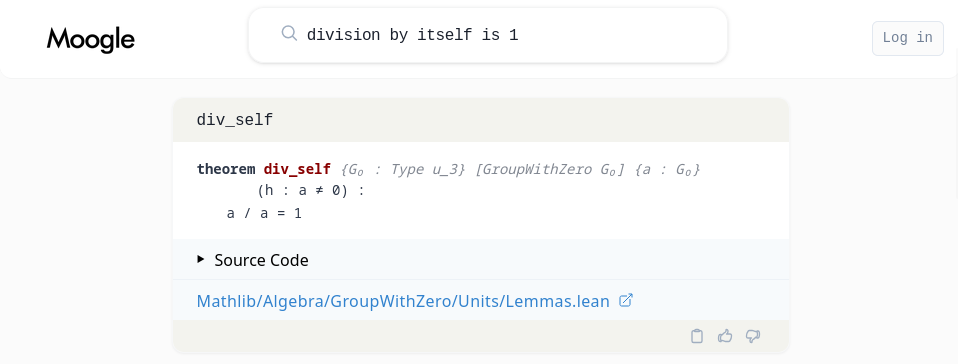
\includegraphics[width=1\textwidth]{figuras/moogle-example.png}
\end{figure}

Que no es el mismo resultado que proponía \bluecode{exact?}, pero parece incluso más simple. Podríamos volver a nuestro ejemplo y escribir

\begin{minipage}[t]{0.58\textwidth}
\begin{lstlisting}[language=lean]
  example (x : ℝ) (hx : x > 0) :
      x / x = 1 := by
    apply div_self

~
\end{lstlisting}
\end{minipage}%
\hfill
\begin{minipage}[t]{0.40\textwidth}
\begin{lstlisting}[language=infoview]
  Tactic state
    ŋ1 goalŋ
    ħxħ : ℝ
    ħhxħ : x > 0
    ⊢ x ≠ 0
\end{lstlisting}
\end{minipage}

Con lo que ya sólo faltaría demostrar que $x \neq 0$.

En general, he encontrado que LeanSearch funciona mejor que Moogle, especialmente en términos de relevancia de los resultados obtenidos. Sin embargo, al principio del proyecto solo conocía Moogle, y descubrí LeanSearch más tarde, por lo que he utilizado Moogle mayoritariamente.

Un ejemplo de una búsqueda real que necesité para el trabajo en LeanSearch, fue \textit{\quotes{subset of set has at most the dimension of the set}}.

\begin{figure}[h]
  \centering
  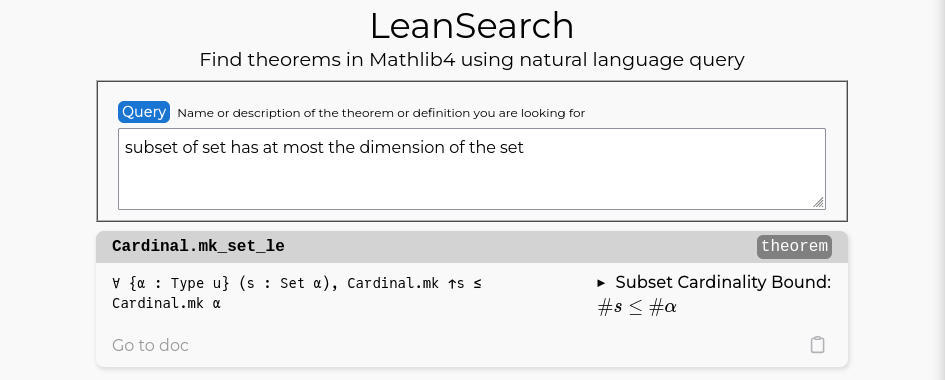
\includegraphics[width=1\textwidth]{figuras/leansearch-example-cropped.png}
\end{figure}

El primer resultado que aparece es justo el que necesitaba. Sin embargo, antes de buscarlo no tenía ninguna idea de cómo formalizar los resultados en los que estaba trabajando, especialmente porque no estaba familiarizada con el módulo \code{Cardinal.mk}. Este fue un ejemplo claro de que estas herramientas permiten acceder a partes de Mathlib que de otro modo serían difíciles de localizar.

En conjunto, herramientas como \bluecode{exact?}, LeanSearch o Moogle han resultado fundamentales para hacer más eficiente el proceso de formalización, permitiendo apoyarse en Mathlib de forma efectiva sin necesidad de conocerla en profundidad desde el principio.


\subsubsection{Noncomputable y el axioma de elección}

Para finalizar esta sección sobre Lean en la práctica, es útil comentar brevemente una cuestión que aparecerá en algunas de las definiciones posteriores: el uso del \textbf{axioma de elección} y la palabra clave \bluecode{noncomputable}.

En Lean, el axioma de elección se introduce de forma directa mediante

\begin{lstlisting}
  axiom choice {α : Sort u} : Nonempty α → α
\end{lstlisting}

Es decir, dado un tipo no vacío, \code{choice} nos devuelve un elemento de ese tipo, aunque no nos dice cómo encontrarlo. Por este motivo, su uso impide extraer información computable del resultado.

En consecuencia, cuando definimos funciones o construcciones que dependen de \code{choice}, Lean nos obliga a marcarlas como \bluecode{noncomputable}.  Un ejemplo es la función \code{choose}, que dada una prueba de tipo existencial, selecciona un testigo:

\begin{lstlisting}
  noncomputable def choose {α : Sort u} {p : α → Prop}
      (h : ∃ x, p x) : α :=
    (indefiniteDescription p h).val
\end{lstlisting}

A menudo utilizaremos \code{choose} (\code{Classical.choose}, ya que se encuentra en el módulo \code{Classical}) en nuestros resultados, junto con el siguiente lema

\begin{lstlisting}
  theorem choose_spec {α : Sort u} {p : α → Prop}
      (h : ∃ x, p x) : p (choose h) :=
    (indefiniteDescription p h).property
\end{lstlisting}

que es una demostración de que el elemento elegido mediante \code{choose} cumple las propiedades que le pedíamos.

El uso de \bluecode{noncomputable} no representa un problema para nosotros (ni, en general, para la comunidad matemática), ya que en este trabajo no nos interesa que las construcciones sean computables: trabajamos con ellas desde un punto de vista lógico y matemático, no algorítmico.

Además, usar el axioma de elección tiene una ventaja práctica: cuando utilicemos \code{choose}, el elemento elegido será siempre el mismo (aunque no sepamos cuál es), y tendrá siempre la propiedad \code{choose\_spec}. Esto permite trabajar con él de forma coherente dentro de una demostración y referirse a él varias veces como si fuera un objeto determinado.
